\DiaryEntry{Huffman Codes, cont'd}{2021-05-03}{Coding}

\subsection{Code Performance}

To demonstrate the performance of Huffman codes, I created a script which creates an alphabet with given size and random symbol probabilities. \todo{add ref}

For $N = 8$ symbols and $10.000$ runs, the mean source entropy is $H \approx 2.736$ bits and the average code word length $l \approx 2.789$. The average difference between code word length and source entropy divided by the source entropy equals $\approx 0.01965$; i.e. we are $2\%$ away from the optimum. The minimum code word length is $1$ bit and maximum code word length is $7$ bits.

The picture is similar for $N = 32$ symbols: Mean source entropy is $H \approx 4.724$ bits and the average code word length $l \approx 4.757$. The average difference between code word length and source entropy divided by the source entropy equals $\approx 0.006845$; i.e. we are $0.6\%$ away from the optimum. The minimum code word length is $3$ bit and maximum code word length is $12$ bits.

The Huffman code procedure assigns short code words (e.g. $1$ bit) only when the symbol probability is very high. It seems that this happens very seldom in the simulation; If we manually tilt the symbol probability of the first symbol to higher values, then we get a minimum code word length of $1$.

As a fun fact, we also note that if we run the Huffman coding procedure with $N = 2^l$ symbols ($l$ being an arbitrary integer) and equal probabilities $1/N$, it produces a "normal" binary code with all symbols having $l$ bits.

\subsection{Canonical Huffman Codes}

It is useful to develop Huffman codes which can be stored in an efficient manner. One way to do this is to write the code in lexicographic order of the symbols. Thus, we first write the code for $a_1$ , then the code for $a_2$, and so on. Each codeword could be represented by the length of the codeword followed by the codeword. 

For the code in Table \ref{2021-04-14_tab1}, we therefore would have $[1, 4, 0001, 2, 4, 0000, 3, 3, 001, \\ 4, 2, 01,  5, 1, 1]$.

This is certainly manageable for the Huffman code of a small alphabet, but it is clearly going to have an impact on compression performance when we have Huffman codes for large alphabets.

We can substantially reduce the storage requirement for the code by using a version of the Huffman code known as the \emph{canonical Huffman code}. We first examine a property of Huffman trees: A Huffman tree is a fully populated tree. That is, there is a codeword assigned to each leaf of the tree (if a codeword is shorter than the longest codeword, the tree below the codeword is pruned; see the previous entry, \ref{2021-04-26:entry}). What we will show is that if we are only given the lengths of the codewords moving from left to right on the tree we can reconstruct the code.

In our running example, the Huffman code has codeword lengths $[4, 4, 3, 2, 1]$. In order to regenerate the code from the lengths, we begin with a tree of depth four (the length of the longest codeword), as shown in the following Figure.

\begin{figure}[H]
    \centering
    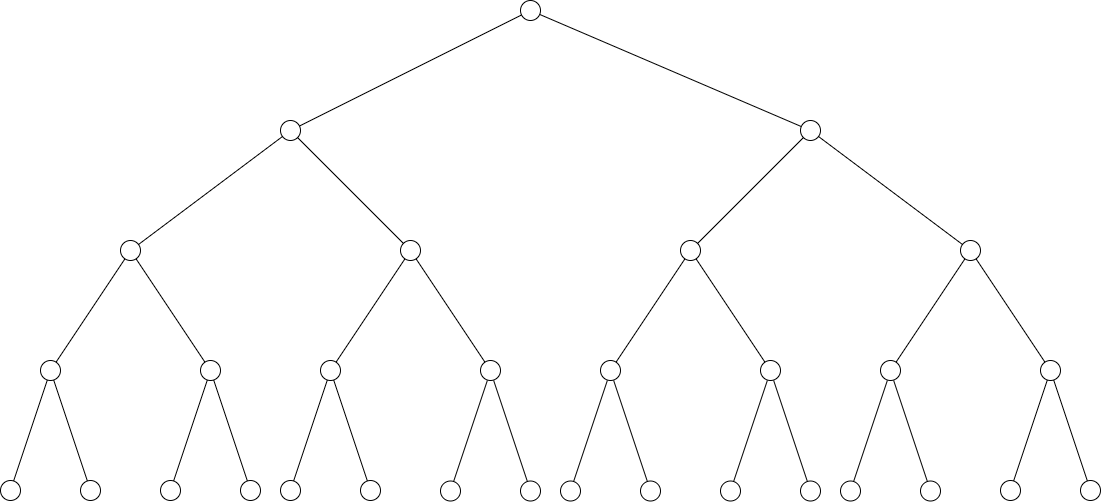
\includegraphics[scale=0.4]{images/2021-05-03_tree_01.png}
\end{figure}


The first codewords have length $4$ so they are located all the way down in the tree. The next codeword has length $3$, so we choose the next "free" node in the tree with length $3$. A Huffman code is a prefix code, we therefore have to prune all nodes below codeword $3$. For the codeword of length $2$ we again choose the next "free" node of length $2$ and prune everything below. Finally, we do the same for the last codeword with length $1$. The resulting tree looks as follows.

\begin{figure}[H]
    \centering
    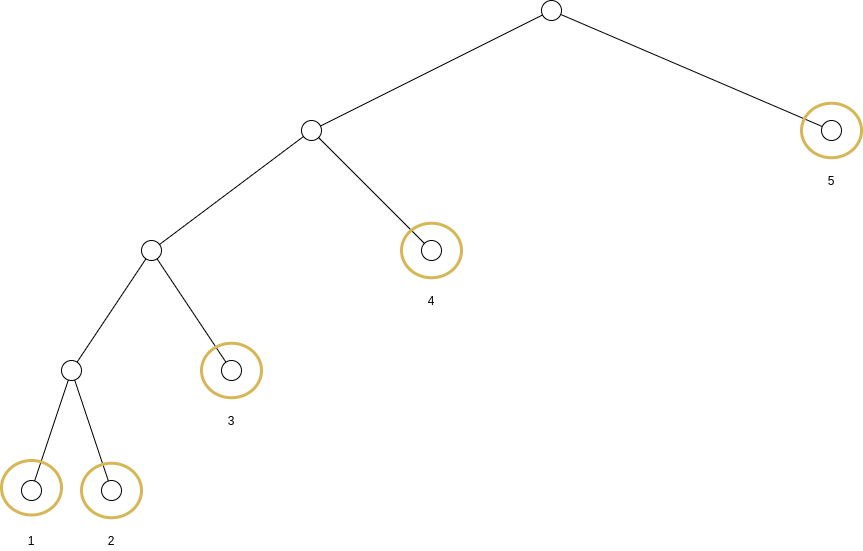
\includegraphics[scale=0.4]{images/2021-05-03_tree_02.png}
\end{figure}

If we assign the left subtree a $1$ and the right subtree a $0$, then we can recover the original code tree and corresponding codewords.So, just knowing the codeword lengths in a particular order permits us to regenerate the Huffman code. The problem is that we do not know which codeword belongs to which letter. The canonical procedure provides us with a way to generate a code that implicitly contains that information. In order to embed this additional information, we need some additional constraints to our Huffman coding procedure. For example, the deflate algorithm in zlib imposes the following conditions on a Huffman code:

\begin{itemize}
    \item All codes of a given length have lexicographically consecutive values in the same order as the symbols they represent.
    \item Shorter codes lexicographically precede longer codes.
\end{itemize}

 Recall that when we generated Huffman codes, we could choose to assign zeros and ones to the branches as we wished. These constraints can be viewed as taking that freedom away.

 We can incorporate these constraints into the Huffman coding procedure, or we can generate a Huffman code using the procedure described previously and transform the code thus produced into a canonical Huffman code. It is simpler to use the latter approach. In order to do this, we will begin by designing a Huffman code. From this design, we will extract the lengths of the codewords. We will use these lengths with the canonical constraints to design the code.

Our example consists of $5$ symbols, $\{a_1, a_2, a_3, a_4, a_5\}$ with codeword lengths $\{4,4,3,2 \\,1\}$. The shortest codeword is assigned to $a_5$, the lexicographically smallest codeword of length one is $0$, so the codeword for $a_5$ is $0$. The codeword of length two has to be of the form $1x$. Since we require only one codeword of length two, we assign $10$ to $a_4$. The codewords of length three now have to be of the form $11x$. We only need a single codeword of length three, the codeword for $a_3$; therefore, the codeword for $a_3$ is $110$. There are two codewords, $a_4$ and $a_5$, of length 4. Therefore, the codeword for $a_4$ is $1110$, and the codeword for $a_5$ is $1111$.

This code can now be encoded by just sending the symbols and their codeword lengths; the actual codewords are \emph{not} required. The resulting codetree is shown in the following Figure.

\begin{figure}[H]
    \centering
    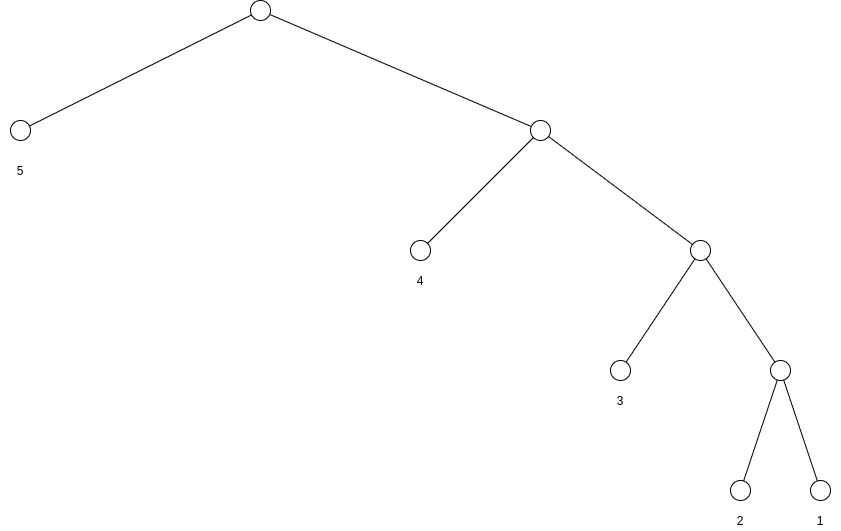
\includegraphics[scale=0.4]{images/2021-05-03_tree_03.png}
\end{figure}


\subsection{Length-limited Huffman Codes}



%%% Local Variables:
%%% mode: latex
%%% TeX-master: "journal"
%%% End:
